\documentclass{article}

\usepackage{amsmath,amssymb}
\usepackage{graphicx}
\usepackage{subfigure}
\usepackage{multirow}
\usepackage{color}
\usepackage{marginnote}
%\usepackage{longtable}

%\usepackage{color}
%\usepackage{listings}

\usepackage{framed}
\usepackage{textpos}

\usepackage[final]{pdfpages}



\renewcommand{\baselinestretch}{1}
\renewcommand{\arraystretch}{1.3}

%you may inactive the following four commands, then it will become appearance of book pages

\setlength{\topmargin}{-0.4in}
%\setlength{\topmargin}{-0.1in}
\setlength{\textheight}{9in}
%\setlength{\textheight}{8.3in}
\setlength{\evensidemargin}{-0.4 in}
\setlength{\oddsidemargin}{-0.4 in}
%\setlength{\oddsidemargin}{0.1 in}
\setlength{\textwidth}{7 in}
%\setlength{\textwidth}{6.2 in}

%%%%%%%%%%%%%

\newtheorem{fact}{Fact}
\newtheorem{algorithm}{Algorithm}
\newtheorem{theorem}{Theorem}
\newtheorem{lemma}{Lemma}
\newtheorem{corollary}{Corollary}
\newtheorem{property}{Property}
\newtheorem{definition}{Definition}
\newtheorem{proposition}{Proposition}
\newtheorem{remark}{Remark}
\newtheorem{conjecture}{Conjecture}

\newcommand{\notsim}{{\, \not \sim \,}}

\newcommand{\F}{\ensuremath{\mathbb F}}
\newcommand{\Z}{\ensuremath{\mathbb Z}}
\newcommand{\N}{\ensuremath{\mathbb N}}
\newcommand{\Q}{\ensuremath{\mathbb Q}}
\newcommand{\R}{\ensuremath{\mathbb R}}
\newcommand{\C}{\ensuremath{\mathbb C}}

\newcommand{\done}{\hfill $\Box$ }
\newcommand{\rmap}{\stackrel{\rho}{\leftrightarrow}}
\newcommand{\mys}{\vspace{0.15in}}

\newcommand{\ebu}{{\bf{e}}}
\newcommand{\Abu}{{\bf{A}}}
\newcommand{\Bbu}{{\bf{B}}}

\newcommand{\abu}{{\bf{a}}}
\newcommand{\abuj}{{\bf{a_j}}}
\newcommand{\bbu}{{\bf{b}}}
\newcommand{\vbu}{{\bf{v}}}
\newcommand{\ubu}{{\bf{u}}}
\newcommand{\dbu}{{\bf{d}}}
\newcommand{\tbu}{{\bf{t}}}
\newcommand{\cbu}{{\bf{c}}}
\newcommand{\kbu}{{\bf{k}}}
\newcommand{\hbu}{{\bf{h}}}
\newcommand{\sbu}{{\bf{s}}}
\newcommand{\wbu}{{\bf{w}}}
\newcommand{\xbu}{{\bf{x}}}
\newcommand{\ybu}{{\bf{y}}}
\newcommand{\zbu}{{\bf{z}}}


\newcommand{\corres}{\leftrightarrow}

\newcommand{\zero}{{\bf{0}}}
\newcommand{\one}{{\bf{1}}}
\newcommand{\nodiv}{{\, \not| \,}}
\newcommand{\notequiv}{{\,\not\equiv\, }}

%%%%%%%%%%%%%%

\def\comb#1#2{{#1 \choose #2}}
\newcommand{\ls}[1]
    {\dimen0=\fontdimen6\the\font\lineskip=#1\dimen0
     \advance\lineskip.5\fontdimen5\the\font
     \advance\lineskip-\dimen0
     \lineskiplimit=0.9\lineskip
     \baselineskip=\lineskip
     \advance\baselineskip\dimen0
     \normallineskip\lineskip\normallineskiplimit\lineskiplimit
     \normalbaselineskip\baselineskip
     \ignorespaces}

\def\stir#1#2{\left\{#1 \atop #2 \right\}}
\def\dsum#1#2{#1 \atop #2 }
\def\defn{\stackrel{\triangle}{=}}

%%%%%%%%



\begin{document}

\thispagestyle{plain}
\setcounter{page}{1}

\begin{center}
{\huge {\bf Indian Institute of Technology, Kharagpur}} 

{\LARGE {\em Department of Computer Science and Engineering}}
\vspace{0.4cm}

{\Large \bf Software Engineering (CS 20006), Spring 2015-16} \vspace{0.1cm}

{\large \bf Postal Management System (PMS)} \vspace{0.1cm}

{\large \em Req. Spec., and Outline of Analysis, and Design} %\vspace{0.3cm}
\end{center}

\hspace{-1cm}

\begin{tabular}{l}
\hspace{16cm} \\ \hline 
\end{tabular}

\begin{enumerate}
\item You are to develop a {\bf Postal Management System (PMS)} for {\em Indian Postal System (IPS)} to assist in its smooth functioning. The requirements specification of the system is given below. Read the specifications carefully, analyse the requirements and design the following aspects of the system using UML and DP. 
\begin{enumerate}
\item \label{Use_Cases} Design suitable Use-Case Diagrams for the specified use-cases. Identify the actors and show the \texttt{$<<$include$>>$}, \texttt{$<<$extend$>>$}, and generalization relationships of the use-cases. %[{\bf 4 Marks}]
\item \label{Select_Classes} Design Class Diagrams for Mails detailing the attributes and operations with their properties. %[{\bf 4 Marks}]
\item Show all other classes / objects (in addition to Question~\ref{Select_Classes}) by brief Class Diagrams (with name and key attributes). For the entire collection of classes (that is, including Mails) show the associations, aggregations/compositions, generalization/specialization, and abstract/concrete etc. %[{\bf 2+2=4 Marks}]
\item Design suitable Sequence Diagrams for any two of the use-cases in Question~\ref{Use_Cases}. %[{\bf 2+2=4 Marks}]
\item Choose appropriate Design Patterns for your design. Briefly justify your choice. %[{\bf 4 Marks}]
\end{enumerate}

\begin{center}
{\bf \underline{Requirements Specification for Postal Management System (PMS)}}
\end{center}

The primary function of {\em Indian Postal System (IPS)} is {\em Collection}, {\em Processing}, {\em Transmission}, and {\em Delivery} of mails. A postal article whose contents are in the nature of message is classified as a Mail. These four stages of mail operation have a single aim -- {\em Delivery of mail to its addressee}. IPS comprises several {\em Post Offices (PO)} and {\em Mail Offices (MO)}. A PO is an end-point of IPS and reaches out to the users of IPS while MOs are intermediate points that ensure proper functioning of IPS by processing, routing, and transmitting mails. Various aspects of IPS, as relevant to PMS, include:

\begin{enumerate}
\item {\em Collection}: Every Mail is collected from a sender and needs to be delivered to a recipient (addressee). Some Mails are collected through {\em Letter-Boxes} while others are collected at counters of a PO. The sender of a Mail may be anonymous while the recipient, naturally, needs to be identified. 

\item {\em Processing}: Mails collected at a PO are first sorted according to their types and certification requirements. The target or destination PO (of the addressee) is then ascertained by the zip code (unique 6-digit number) and the mails are grouped by the required routing for their transmission.

\item {\em Transmission}: Mails for a target PO are then transmitted through the optimal route via one or more MOs using the vehicles of the postal department, and Railway \& Airway Mail Services and finally again using the vehicles of the postal department. 

\item {\em Delivered}: Mails as received at a target PO is delivered to the {\em Mail-Box} of the addressee through postmen who travel to the address on foot or by using bicycles or motor bikes.

\item {\em Certifications}: While the IPS assures delivery of every Mail that it collects, a sender may acquire certified guarantees of collection (of a Mail by PO for delivery) and / or of delivery (of a Mail to the recipient). Certified guarantees are provided in terms of {\em Under Certificate of Posting (UCP)} for collection of a Mail by PO, and as a {\em Registered Letter (RL)} for delivery of a Mail to the recipient. A mail without any certified guarantee is called an {\em Ordinary Mail}.

\item {\em Charges}: PO charges various fees for its services. The charge is decided based on the type of a Mail (as described below), its weight, and requirements of certificates of guarantees. No charge depends on the geographic location of the sender and / or the recipient.

\item The types of Mails handled by IPS are:

\begin{itemize}
\item {\em Post Card (PC)}: A PC is an open communication on a card of prescribed size. It is available in two varieties: {\em Single} \& {\em Reply Post Card (RPC)}. PCs are for transmission within India only. A single PC costs Re. 1/00 and and an RPC costs Rs. 1/50. A recipient can use an RPC to reply without any separate charge. A PC is collected at a letter box. 

No certificates of guarantee is available for a PC. 

\item {\em Inland Letter Card (ILC)}: An ILC is a communication contained on a sheet of paper with prescribed size \& folding. ILCs are used for transmission within India only. An ILC costs Rs. 2/50 and the maximum allowed weight of an ILC is 10 Grams. An ILC is collected at a letter box.

No certificate of guarantee is available for an ILC. 

\item {\em Letter}: A Letter is a communication enclosed in an envelope and addressed. The maximum allowed weight of a Letter is 2 Kilograms. The minimum cost of a Letter is Rs. 5/00 for weight up to 100 Grams. Thereafter Re. 1/00 is charged for every additional 100 Grams. The charge for a Letter is paid through {\em Postage Stamps} of various denominations. A Letter is collected at a counter of a PO.

By default a Letter is an Ordinary Mail. However, a sender of bulk volume of mails may enrol with a PO and can send letters Under Certificate of Posting (UCP). With UCP, the collecting PO issues a certificate to the sender indicating that a letter for the intended recipient has indeed been collected. In addition, a letter can also be sent as a Registered Letter (RL). When an RL is delivered to the recipient, an acknowledgement card is signed by the addressee indicating its receipt. Subsequently the receipt is returned to the sender as a proof of delivery. 

While UCP only has annual enrolment fee of Rs. 100/00, an RL costs Rs. 10/00 extra over an ordinary mail.
 
\item {\em Parcel}: Anything can be sent in a Parcel excepting articles whose transmission is prohibited. It can contain a single communication to the addressee of the Parcel. A Parcel is collected at a counter of a PO.

Like letters, a Parcel can be ordinary (unregistered) or registered. However, there is no UCP available for parcels.

The minimum cost of a Parcel is Rs. 50/00 for weight up to 1 Kilogram. Thereafter Rs. 10/00 is charged for every additional 500 Grams. The charge for a Parcel is paid through {\em Postage Stamps} of various denominations. The maximum allowed weight of an Unregistered Parcel is 4 Kilograms and of a Registered Parcel is 20 Kilograms. A Registered Parcel costs Rs. 100/00 extra over an unregistered one.

\end{itemize}

\item {\em People}: The following persons are involved in the IPS:

\begin{itemize}
\item Sender
\item Recipient
\item Postal Staff (PS) -- working at the counters and back-office of a PO or an MO.
\item Postman -- reaching the recipients.
\end{itemize}

\item {\em Use Cases}: Common use cases of PMS include:
\begin{itemize}
\item [{\em Collection}:] A Sender posts a mail at a letter box or at a PO. The mail may be ordinary or registered. While collecting a mail at a PO, the PS needs to check for correct denominations of postage stamps according to the type and weight of a mail.
\item [{\em Processing}:] Postal Staffs process mails. This includes sorting the mails according to type of mail, whether registered or not, and the address (zip code). Mails going to a common PO or MO are put in a postal bag. 
\item [{\em Transmission}:] Mails (in postal bags) are transmitted through POs and MOs. Once an MO receives a postal bag, it needs to forward it to the next MO or PO. A PO only receives the bag of mails for addresses within the zip code of the PO.
\item [{\em Delivery}:] A Postman delivers a mail. A Recipient receives a mail in her Mail Box or in person. For a registered mail the Postman gets the signature of the recipient on the acknowledgement card which in turn is delivered to the Sender.
\end{itemize}

\end{enumerate}


\end{enumerate}



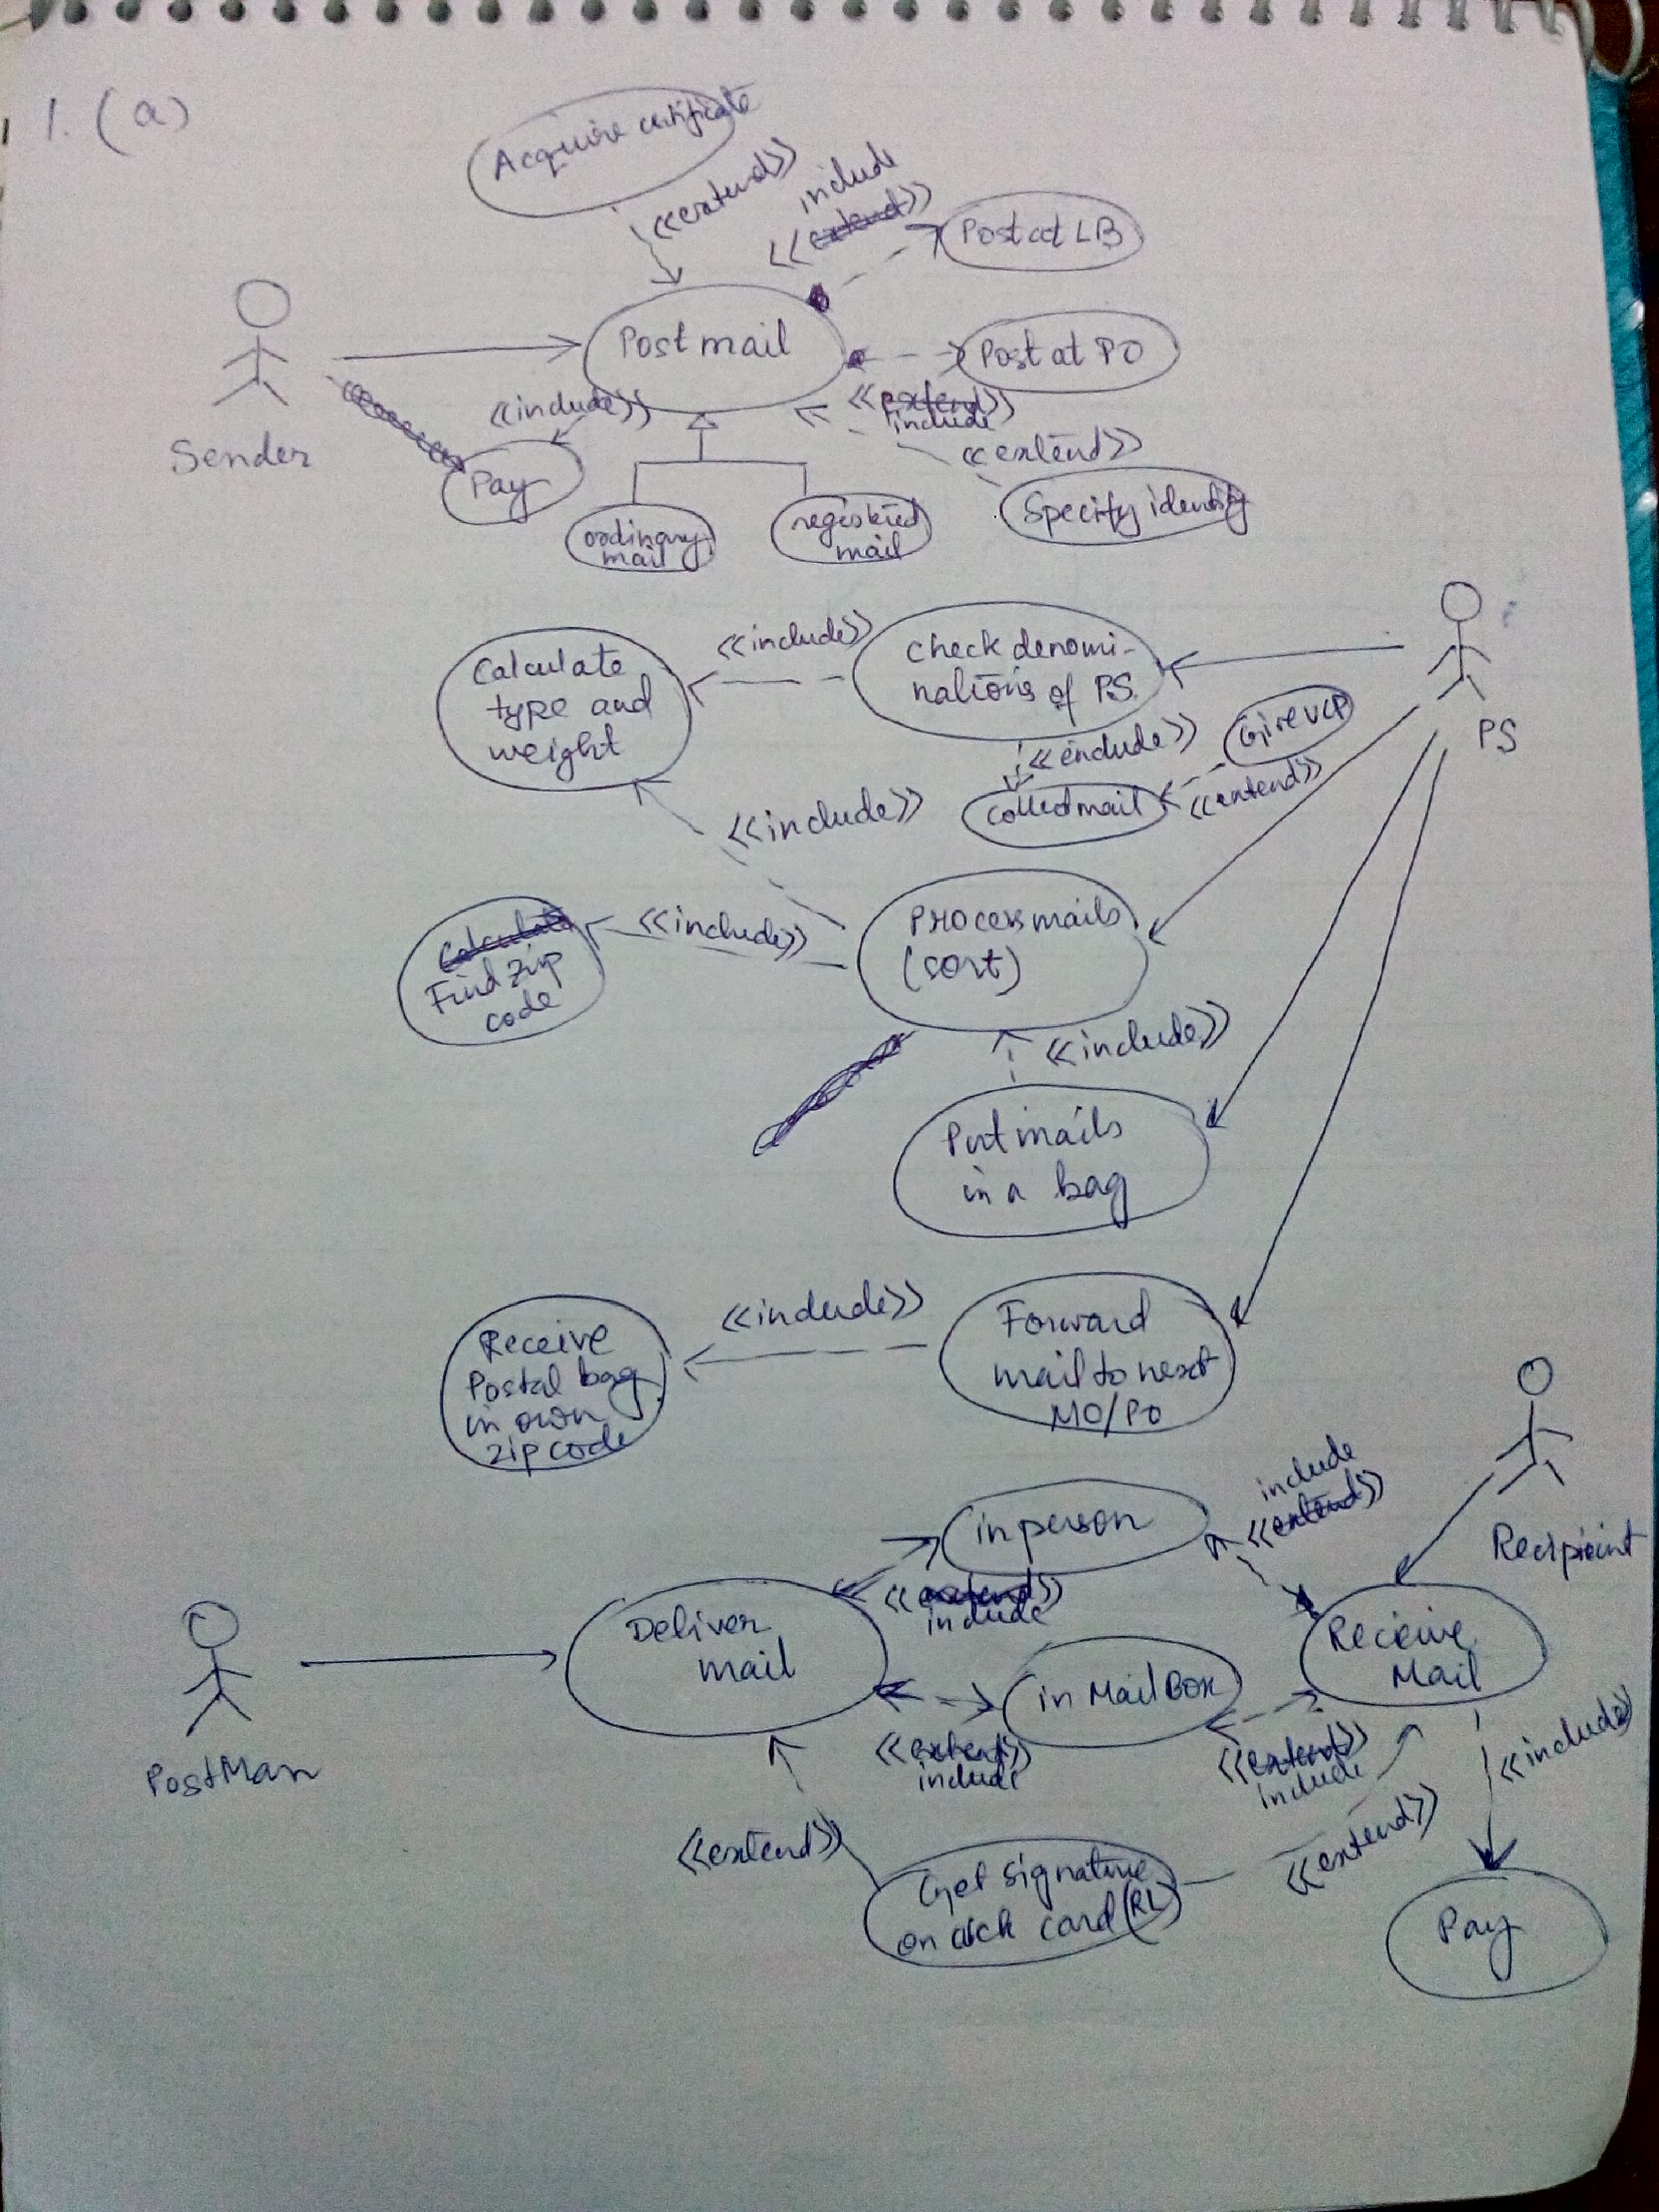
\includepdf[width=15cm, pages=-]{PMS_Solution.pdf}
\end{document}
